\documentclass[11pt,onecolumn,journal]{IEEEtran}
\usepackage{}
\usepackage{mathrsfs}
\usepackage{bbm}
\usepackage{amsfonts}
\usepackage{amsmath}
\usepackage{cases}%���������{amsmath}����
\newcounter{mytempeqncnt}
\usepackage{amssymb}
\usepackage{booktabs}
\usepackage{graphicx}

\usepackage{algorithm}
\usepackage{algorithmic}
\usepackage{setspace}
%\doublespacing
\usepackage{dsfont}

%\usepackage{tikz}
\hyphenation{op-tical net-works semi-conduc-tor}
\newcommand\old[1]{}
\def\bi{\bibitem}
\newcommand{\bm}[1]{\mbox{\boldmath{$#1$}}}
\renewcommand{\baselinestretch}{1.5}
\newtheorem{definition}{Definition}
%\newtheorem{algorithm}{Algorithm}
\newtheorem{lemma}{Lemma}
\newtheorem{corollary}{Corollary}
\newtheorem{proposition}{Proposition}
\newtheorem{theorem}{Theorem}
\newtheorem{remark}{Remark}
\newtheorem{example}{Example}
\newtheorem{assumption}{Assumption}
%\newtheorem{practitioners}{Note to Practitioners}
%\newtheorem{practitioners}{Note to Practitioners}

\begin{document}


\title{Chapter 5}

\maketitle

\textbf{5.1  Is the network shown in Fig. 5.2 BIBO stable? If not, find a bounded input that will excite an unbounded output.}\\
\begin{figure}[hp]
\centering
    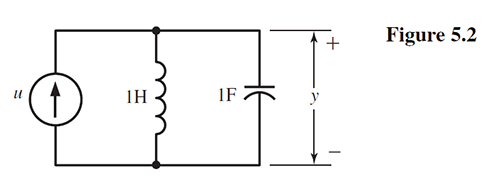
\includegraphics{p51.png}
    \end{figure}

\textbf{Solution:}\\

The transfer function of the system is \\
\begin{center}
    \begin{eqnarray*}\begin{split}
    g(s)&=\frac{s\cdot \frac{1}{s}}{s+\frac{1}{s}}\\
    &=\frac{s}{s^2+1}
    \end{split}\end{eqnarray*}
\end{center}

Let $u(t)=\sin(t)$,then the Laplace transform of $u(t)$ is $u(s)=\frac{1}{s^2+1}$,and the output will be \\
\begin{center}
    $y(s)=\frac{s}{(s^2+1)^2}$
\end{center}

By inverse Laplace transform,we have $y(t)=0.5t\sin(t)$,and it is not bounded.So the system is not BIBO stable.\\

\textbf{5.2 Consider a system with an irrational transfer function }$\hat{g}(s)$. \textbf{Show that a necessary condition for the system to be BIBO stable is that} $|\hat{g}(s)|$ \textbf{is finite for all Re} $s \geq 0$.\\

\textbf{Solution:}\\

$g(s)=\int_0^\infty g(t)e^{-st} dt$.And let $s=\sigma +j\omega$,then we have:\\
\begin{center}
    \begin{eqnarray*}\begin{split}
    \left|e^{-st}\right|&=\left|e^{-\sigma t}\right|\left|e^{-j\omega t}\right|\\
    &=\left|e^{-\sigma t}\right|\\
    &\leq1
    \end{split}\end{eqnarray*}
\end{center}

So if the system is BIBO stable,then we have $\int_0^\infty \left|g(t)\right| dt < \infty$,thus we have for $Re>0$\\
\begin{center}
    $\left|g(s)\right|\leq \int_0^\infty \left|g(t)\right|\left|e^{-st}\right| dt\leq \int_0^\infty \left|g(t)\right| dt \leq \infty$.Thus the necessarily can be proved.
\end{center}

\textbf{5.3 Is a system with impulse response }$g(t)=1 /(t+1)$ \textbf{BIBO stable? How about} $g(t)=t e^{-t}$\textbf{ for }$t \geq 0 ?$\\

\textbf{Solution:}\\

For $g(t)=1 /(t+1)$:\\
\begin{center}
\begin{eqnarray*}\begin{split}
\int_0^\infty \left|g(t)\right| dt &=\int_0^\infty\left|1 /(t+1)\right| dt\\
&=\left.ln(t+1)\right|^\infty_0\\
&=\infty
\end{split}\end{eqnarray*}
\end{center}

So $g(t)$ is not absolutely integrable,the system is not BIBO stable.\\

For $g(t)=t e^{-t}$:\\
By taking Laplace transform,$g(s)=\frac{1}{(s+1)^2}$,and all the roots have negative real parts,so the system is BIBO stable.\\

\textbf{5.4 Is a system with transfer function }$\hat{g}(s)=e^{-2 s} /(s+1)$ \textbf{BIBO stable?}\\

\textbf{Solution:}\\

By taking Laplace transform,we have\\
\begin{center}
    For $t\geq 2$,$g(t)=e^{-t+2}$\\
    For $t<2$,$g(t)=0$
\end{center}

Then\\
\begin{center}
    \begin{eqnarray*}\begin{split}
    \int_0\infty \left|g(t)\right| dt&=\int_2\infty \left|e^{-t+2}\right| dt\\
    &=\left.-e^{-t+2}\right|_2^\infty\\
    &=1
    \end{split}\end{eqnarray*}
\end{center}
So $g(t)$ is absolutely integrable,and the system is BIBO stable.\\

\textbf{5.5 Show that the negative-feedback system shown in Fig. 2.5 (b) is BIBO stable if and only if the gain a has a magnitude less than 1. For }$a=1,$ \textbf{find a bounded input} $r(t)$ \textbf{that will excite an unbounded output.}\\

\textbf{Solution:}\\

If $r(t)=\delta (t)$,then we have $g(t)=a\delta(t-1)-a^2\delta(t-2)+a^3\delta(t-3)+\cdots $.And\\
\begin{center}
    \begin{eqnarray*}\begin{split}
    \int_0^\infty \left|g(t)\right| dt&=\int_0^\infty \left|a\delta(t-1)-a^2\delta(t-2)+a^3\delta(t-3)+\cdots\right| dt\\
    &=|a|+|a|^2+|a|^3+\cdots\\
    &=\left\{\begin{array}{l}\frac{|a|}{1-|a|},|a|<1\\
    \infty,|a|\geq 1\end{array}\right.
    \end{split}\end{eqnarray*}
\end{center}

So the system is BIBO stable if $|a|<1$.\\

And if $a=1$,let $r(t)=\left\{\begin{array}{ll} 1 & 2n<t<2n+1,n=0,1,2,\cdots\\
-1 & 2n+1<t<2n+2,n=0,1,2,\cdots\end{array}\right.$.Obviously $r_m=1<\infty$,so the input is bounded.\\

Then the output will be $y(t)=i\times (-1)^{i+1},i<t<i+1,i=0,1,2,\cdots$,and the output is not bounded.So the system is not BIBO stable.\\

\textbf{5.6 Consider a system with transfer function }$\hat{g}(s)=(s-2) /(s+1)$. \textbf{What are the steady-state responses excited by} $u(t)=3,$ \textbf{for} $t \geq 0,$ \textbf{and by} $u(t)=\sin 2 t,$ \textbf{for} $t \geq 0 ?$\\

Solution:\\

From theorem 5.2,we have\\

For $u(t)=3$,$y(t)=3\times \hat{g}(0)=-6$\\

For $u(t)=\sin(2t)$,$y(t)=\left|\hat{g}(j2)\right|\sin(2t+\varphi (\hat{g}(j2)))=1.26\sin(t+1.25)$\\

\textbf{5.7 Consider}
$$
\begin{array}{l}
\dot{\mathbf{x}}=\left[\begin{array}{rr}
-1 & 10 \\
0 & 1
\end{array}\right] \mathbf{x}+\left[\begin{array}{c}
-2 \\
0
\end{array}\right] u \\
y=[-2 \quad 3] \mathbf{x}-2 u
\end{array}
$$

\textbf{Is it BIBO stable?}\\

\textbf{Solution:}\\

The transfer function is\\
\begin{center}
    \begin{eqnarray*}\begin{split}
    g(s)&=\left[\begin{array}{ll} -2 & 3\end{array}\right]\left[\begin{array}{ll}-1 & 10\\0 & 1\end{array}\right]^{-1}\left[\begin{array}{l} -2\\0\end{array}\right]\\
    &=\frac{4}{s+1}
    \end{split}\end{eqnarray*}
\end{center}

The root of the transfer matrix has negative real part,so the system is BIBO stable.\\

\textbf{5.8 Consider a discrete-time system with impulse response sequence}
$$
g[k]=k(0.8)^{k} \quad \text { for } k \geq 0
$$
\textbf{Is the system BIBO stable?}\\

\textbf{Solution:}\\

By taking z-transform,we have\\
\begin{center}
    $g(z)=\frac{0.8z}{(z-0.8)^2}$
\end{center}

Then the poles lie in the unit circle,so the system is BIBO stable.\\

\textbf{5.9 Is the state equation in Problem 5.7 marginally stable? Asymptotically stable?}\\

\textbf{Solution:}\\

$\lambda I-A=\left[\begin{array}{ll}\lambda+1 & \lambda-10\\0 & \lambda -1\end{array}\right]$,so the eigenvalues are -1 and 1.Since there is one eigenvalue 1 that has positive real part,the system is neither marginally stable nor asymptotically stable.\\

\textbf{5.10 Is the homogeneous state equation}
$$
\dot{\mathbf{x}}=\left[\begin{array}{rrr}
-1 & 0 & 1 \\
0 & 0 & 0 \\
0 & 0 & 0
\end{array}\right] \mathbf{x}
$$
\textbf{marginally stable? Asymptotically stable?}\\

\textbf{Solution:}\\

$\lambda I-A=\left[\begin{array}{lll}\lambda+1 & 0 & -1\\0 & \lambda & 0\\0 & 0 &\lambda\end{array}\right]$,and by the determinant of it we can get that the eigenvalues of A are 0,0,-1.Thus the system is not asymptotically stable.Then for eigenvalue 0,let $\lambda=0$,then $(\lambda I-A)x=0$ will be\\
\begin{center}
    $\left[\begin{array}{lll}1 & 0 & -1\\0 & 0 & 0\\0 & 0 & 0\end{array}\right]x=0$
\end{center}

The coefficient matrix has rank 1,so there are 2 independent solutions.So matrix A can be transformed as $\left[\begin{array}{lll}-1 & 0 & 0\\0 & 0 & 0 \\0 & 0 & 0\end{array}\right]$.And the minimal polynomial is $\lambda(\lambda+1)$,so 0 is the single root of the minimal polynomial.Thus the system is marginally stable.\\

\textbf{5.11 Is the homogeneous state equation}
$$
\dot{\mathbf{x}}=\left[\begin{array}{rrr}
-1 & 0 & 1 \\
0 & 0 & 1 \\
0 & 0 & 0
\end{array}\right] \mathbf{x}
$$
\textbf{marginally stable? Asymptotically stable?}\\

\textbf{Solution:}\\

$\lambda I-A=\left[\begin{array}{lll}\lambda +1 & 0 & -1\\0 & 0 & \lambda-1\\0 & 0 & \lambda\end{array}\right]$,so the characteristic polynomial is $\lambda^2(\lambda+1)$,the eigenvalues are 0,0,-1.Thus the system is not asymptotically stable.For eigenvalue 0,$(\lambda I-A)x=0$ will be \\
\begin{center}
    $\left[\begin{array}{lll}1 & 0 & -1\\0 & 0 & -1\\0 & 0 & 0\end{array}\right]x=0$
\end{center}

The coefficient matrix has rank 2,so there is only 1 independent solution.The solution will be $\left[\begin{array}{lll}0 & 1 & 0\end{array}\right]'$,and from this there exists a generated solution $\left[\begin{array}{lll} 1 & 0 & 1\end{array}\right]'$.These two vectors consists of the eigenvectors of eigenvalue 0.And from the calculation we can get that A can be transform as $\left[\begin{array}{lll}-1 & 0 & 0\\0 & 0 & 1\\0 & 0 & 0\end{array}\right]$.So the minimal polynomial will be $\lambda^2(\lambda+1)$,and since 0 is not single root of the minimal polynomial,the system is not marginally stable.\\

\textbf{5.12 Is the discrete-time homogeneous state equation}
$$
\mathbf{x}[k+1]=\left[\begin{array}{rrr}
0.9 & 0 & 1 \\
0 & 1 & 0 \\
0 & 0 & 1
\end{array}\right] \mathbf{x}[k]
$$
\textbf{marginally stable? Asymptotically stable?}\\

\textbf{Solution:}\\

The eigenvalues of A are 0.9,1,1.So the system is not asymptotically stable.Then for eigenvalue 1,$I-A$ has rank 1,so there are two independent solutions for $(I-A)x=0$.So A can be transformed into\\
\begin{center}
    $\left[\begin{array}{lll}0.9 & 0 & 0\\0 & 1 & 0\\ 0 & 0 & 1\end{array}\right]$
\end{center}

And the minimal polynomial will be $(\lambda-1)(\lambda-0.9)$,so 1 is the single root of the minimal polynomial.So the system is marginally stable.\\

\textbf{5.13 Is the discrete-time homogeneous state equation}
$$
\mathbf{x}[k+1]=\left[\begin{array}{rrr}
0.9 & 0 & 1 \\
0 & 1 & 1 \\
0 & 0 & 1
\end{array}\right] \mathbf{x}[k]
$$
\textbf{marginally stable? Asymptotically stable?}\\

\textbf{Solution:}\\

The characteristic polynomial is $(\lambda-1)^2(\lambda-0.9)$.So the system is not asymptotically stable.As for eigenvalue 1,$I-A$ will be\\
\begin{center}
    $\left[\begin{array}{lll}0.1 & 0 -1\\0 & 0 & -1 \\0 & 0 & 0\end{array}\right]$
\end{center}

The coefficient matrix has rank 2.So there is only one independent solution for $(I-A)x=0$.Thus A can be transformed into\\
\begin{center}
    $\left[\begin{array}{lll} 0.9 & 0 & 0\\0 & 1 & 1\\0 & 0 & 1\end{array}\right]$
\end{center}

From the Jordan form,we can get that the minimal polynomial of A is $(\lambda-1)^2(\lambda-0.9)$.So 1 is not the single root of the minimal polynomial.The system is not marginally stable.\\

\textbf{5.14 Use Theorem 5.5 to show that all eigenvalues of}
$$
\mathbf{A}=\left[\begin{array}{rr}
0 & 1 \\
-0.5 & -1
\end{array}\right]
$$
\textbf{have negative real parts.}\\

\textbf{Solution:}\\

As for the Lyapunov equation $A'M+MA=-N$,we can choose N to be identity matrix.Then the equation will be\\
\begin{center}
    $\left[\begin{array}{ll}0 & -0.5\\1 & -1\end{array}\right]\left[\begin{array}{ll}m_{11} & m_{12}\\m_{21} & m_{22}\end{array}\right]+\left[\begin{array}{ll}m_{11} & m_{12}\\m_{21} & m_{22}\end{array}\right]\left[\begin{array}{ll}0 & 1\\-0.5 & -1\end{array}\right]=\left[\begin{array}{ll}-1 & 0\\0 & -1\end{array}\right]$
\end{center}

And by solving the equation,we can get $M=\left[\begin{array}{ll} 1.75 & 1\\1 & 1.5\end{array}\right]$.Since $1.75>0$,$1.75\times 1.5-1>0$,M is of positive definite.So all eigenvalues of A have negative real parts.\\

\textbf{5.15 Use Theorem 5.D5 to show that all eigenvalues of the A in Problem 5.14 have magnitudes less than 1.}\\

\textbf{Solution:}\\

For the Lyapunov equation $M-A'MA=N$,we choose N to be identity matrix.Then we have\\
\begin{center}
    $\left[\begin{array}{ll}m_{11} & m_{12}\\m_{21} & m_{22}\end{array}\right]-\left[\begin{array}{ll}0 & -0.5\\1 & -1\end{array}\right]\left[\begin{array}{ll}m_{11} & m_{12}\\m_{21} & m_{22}\end{array}\right]\left[\begin{array}{ll}0 & 1\\-0.5 & -1\end{array}\right]=\left[\begin{array}{ll}1 & 0\\0 & 1\end{array}\right]$
\end{center}

By solving the equation,we can get that $M=\left[\begin{array}{ll}2.2 & 1.6\\1.6 & 4.8\end{array}\right]$.The matrix is of positive definite,so all eigenvalues of the A have magnitudes less than 1.\\

\textbf{5.16 For any distinct negative real }$\lambda_i$ \textbf{and any nonzero real} $a_i$ , \textbf{show that the matrix}
$$
\mathbf{M}=\left[\begin{array}{rrr}
-\frac{a_{1}^{2}}{2 \lambda_{1}} & -\frac{a_{1} a_{2}}{\lambda_{1}+\lambda_{2}} & -\frac{a_{1} a_{3}}{\lambda_{1}+\lambda_{3}} \\
-\frac{a_{2} a_{1}}{\lambda_{2}+\lambda_{1}} & -\frac{a_{2}^{2}}{2 \lambda_{2}} & -\frac{a_{2} a_{3}}{\lambda_{2}+\lambda_{3}} \\
-\frac{a_{3} a_{1}}{\lambda_{3}+\lambda_{1}} & -\frac{a_{3} a_{2}}{\lambda_{3}+\lambda_{2}} & -\frac{a_{3}^{2}}{2 \lambda_{3}}
\end{array}\right]
$$
\textbf{is positive definite. [Hint: Use Corollary 5.5 and }$\mathbf{A}=\operatorname{diag}\left(\lambda_{1}, \lambda_{2}, \lambda_{3}\right)$\textbf{.]}\\

\textbf{Solution:}\\

Let $\mathbf{A}=\operatorname{diag}\left(\lambda_{1}, \lambda_{2}, \lambda_{3}\right)$,then the Lyapunov equation will be \\
\begin{center}
    $-\left[\begin{array}{lll}a_1^2 & a_1a_2 & a_1a_3\\a_1a_2 & a_2^2 & a_2a_3\\a_1a_3 & a_2a_3 & a_3^2\end{array}\right]=-N$
\end{center}

Let $N=\bar{N}'\bar{N}$,then we have $\bar{N}=\left[\begin{array}{lll} a_1 & a_2 & a_3\end{array}\right]$.Then construct the following matrix:\\
\begin{center}
    $\left[\begin{array}{l}\bar{N}\\ \bar{N}A \\ \bar{N}A^2\end{array}\right]=\left[\begin{array}{lll} a_1 & a_2 & a_3\\ \lambda_1a_1 & \lambda_2a_2 & \lambda_3a_3\\ \lambda^2_1a_1 & \lambda^2_2a_2 & \lambda^2_3a_3\end{array}\right]\doteq \alpha$.
\end{center}

And $\det (\alpha)=a_1a_2a_3(\lambda_3-\lambda_1)(\lambda_3-\lambda_2)(\lambda_2-\lambda_1)$.Since $a_i$ are all non-zero,and $\lambda_i$ are all distinct,$\det \alpha \neq 0$.So $\alpha$ is of full rank and from the corollary M is of positive definite.\\

\textbf{5.17 A real matrix }$\mathbf{M}$ \textbf{(not necessarily symmetric) is defined to be positive definite if} $\mathbf{x}^{\prime} \mathbf{M} \mathbf{x}>0$ \textbf{for any nonzero} $\mathbf{x}$. \textbf{Is it true that the matrix} $\mathbf{M}$ \textbf{is positive definite if all eigenvalues of} $\mathbf{M}$ \textbf{are real and positive or if all its leading principal minors are positive? If not, how do you check its positive definiteness? [Hint: Try}
$$
\left[\begin{array}{cc}
0 & 1 \\
-2 & 3
\end{array}\right] \quad\left[\begin{array}{cc}
2 & 1 \\
1.9 & 1
\end{array}\right]]
$$

\textbf{Solution:}\\

Let $H_1=\left[\begin{array}{cc}
0 & 1 \\
-2 & 3
\end{array}\right]$,$H_2=\left[\begin{array}{cc}
2 & 1 \\
1.9 & 1
\end{array}\right]$.\\

For matrix $H_1$,the eigenvalues are $1,2$.Let $x=\left[\begin{array}{ll}4 & 1\end{array}\right]'$,then $x'Ax=-1<0$,so the matrix is not positive definite.\\

For matrix $H_2$,let $x=\left[\begin{array}{ll} 0.5805 & -0.8142\end{array}\right]$.And $x'Ax=-0.0338<0$.The matrix is not positive definite.But all its leading principal minors are 2 and 0.1.They are both larger than 0.\\

So we cannot judge the positive definiteness of the matrix by eigenvalues or leading principal minors if matrix is not symmetric.\\

Under this condition,we can construct matrix $\hat{H}=\frac{1}{2}(H'+H)$.That is,for matrix $H_1$,$H_1^{\prime}=\left[\begin{array}{ll} 0 & -0.5\\-0.5 & 3\end{array}\right]$.It is not positive definite because the leading principal minors are 0,-0.25.Similarly,$H_2^{\prime}=\left[\begin{array}{ll} 2 & 1.45\\1.45 & 1\end{array}\right]$.It is not positive definite since the leading principal minors are 2,-0.1025.\\

\textbf{5.18 Show that all eigenvalues of A have real parts less than} $-\mu<0$ \textbf{if and only if, for any given positive definite symmetric matrix} $\mathbf{N},$ \textbf{the equation}
$$
\mathbf{A}^{\prime} \mathbf{M}+\mathbf{M} \mathbf{A}+2 \mu \mathbf{M}=-\mathbf{N}
$$
\textbf{has a unique symmetric solution }$\mathbf{M}$ \textbf{and} $\mathbf{M}$ \textbf{is positive definite.}\\

\textbf{Solution:}\\

The equation can be transformed as:\\
\begin{center}
    $(A'+\mu I')M+M(A+\mu I')=-N$
\end{center}

Since the equation has a unique symmetric solution M and M is positive definite for any given positive definite symmetric matrix N,$(A+\mu I)$ has eigenvalues with negative real parts.Let the eigenvalues of A be $\lambda_i$,then the eigenvalues of $A+\mu I$ can be $\lambda+\mu$.Then we have $Re(\lambda)<-\mu$.\\

\textbf{5.19 Show that all eigenvalues of A have magnitudes less than $\rho$ if and only if, for any given positive definite symmetric matrix} $\mathbf{N},$ \textbf{the equation}
$$
\rho^{2} \mathbf{M}-\mathbf{A}^{\prime} \mathbf{M} \mathbf{A}=\rho^{2} \mathbf{N}
$$
\textbf{has a unique symmetric solution} $\mathbf{M}$ \textbf{and} $\mathbf{M}$ \textbf{is positive definite.}\\

\textbf{Solution:}\\

The equation can be transformed as:\\
\begin{center}
    $M-(\frac{1}{\rho}A')M(\frac{1}{\rho}A)=N$
\end{center}

If $N>0,M>0$,then we can get that all the eigenvalues of $\frac{1}{\rho}A$ have magnitudes less than 1.Let $\lambda_i$ be the eigenvalues of A,then we have $\left|\frac{1}{\rho}\lambda_i\right|<1$,that is,$\left|\lambda_i\right|<\rho$.\\

\textbf{5.20 Is a system with impulse response }$g(t, \tau)=e^{-2|t|-|\tau|},$ \textbf{for} $t \geq \tau,$ \textbf{BIBO stable? How about} $g(t, \tau)=\sin t\left(e^{-(t-\tau)}\right) \cos \tau ?$\\

\textbf{Solution:}\\
$g(t, \tau)=e^{-2|t|-|\tau|}:$\\

By integration,we have:\\
\begin{center}
    $\int_{t_0}^t |e^{-2|t|-|\tau|}| d\tau=e^{-2|t|}\int_{t_0}^t e^{-|\tau|} d\tau\doteq \alpha$
\end{center}
When $t_0\leq t <0$,we have:\\
\begin{center}
    \begin{eqnarray*}\begin{split}
    e^{-2|t|}\int_{t_0}^t e^{-|\tau|} d\tau&=e^{2t}\int_{t_0}^t e^{\tau} d\tau\\
    &=e^{2t}(e^t-e^{t_0})\\
    &<\infty
    \end{split}\end{eqnarray*}
\end{center}

When $t_0\leq t,t>0$,we have:\\
\begin{center}
    \begin{eqnarray*}\begin{split}
    \alpha&=e^{-2t}(\int_{t_0}^0 e^{\tau} d\tau+\int_0^t e^{-\tau} d\tau)\\
    &=e^{-2t}[(1-e^{t_0})-(e^{-t}-1)]\\
    &=e^{-2t}(-e^{-t}-e^{t_0}+2)\\
    &<\infty(t_0<0)
    \end{split}\end{eqnarray*}
\end{center}
\begin{center}
    \begin{eqnarray*}\begin{split}
    \alpha&=e^{-2t}\int_{t_0}^t e^{-\tau} d\tau\\
    &=e^{-2t}(e^{-t_0}-e^{-t})\\
    &<\infty(t_0>0)
    \end{split}\end{eqnarray*}
\end{center}

So the system is BIBO stable.\\

$g(t, \tau)=\sin t\left(e^{-(t-\tau)}\right) \cos \tau :$\\

With integration,we have:\\
\begin{center}
    \begin{eqnarray*}\begin{split}
    \int_{t_0}^{\infty} |g(t-\tau)| d\tau &\leq \int_{t_0}^{t} e^{-(t-\tau)} d\tau\\
    &=e^{-t}\int_{t_0}^t e^{\tau} d\tau\\
    &=e^{-t}(e^{t}-e^{t_0})\\
    &=1-e^{-(t-t_0)}\\
    &<\infty
    \end{split}\end{eqnarray*}
\end{center}

So the system is BIBO stable.\\

\textbf{5.21 Consider the time-varying equation}
$$
\dot{x}=2 t x+u \quad y=e^{-t^{2}} x
$$
\textbf{Is the equation BIBO stable? Marginally stable? Asymptotically stable?}\\

\textbf{Solution:}\\

For the scalar equation,we have:\\
\begin{center}
    $\phi (t,t_0)=e^{\int_{t_0}^t e^{2t} dt}=e^{t^2-t_0^2}$
\end{center}

Thus $g(t,\tau)=e^{-\tau^2}$,and with integration,we have:\\
\begin{center}
    \begin{eqnarray*}\begin{split}
    \int_{t_0}^t|g(t,\tau)| d\tau&=\int_{t_0}^t e^{-\tau^2} d\tau\\
    &<\infty
    \end{split}\end{eqnarray*}
\end{center}

Since $e^{-\tau^2}<e^{-\tau}<\infty$ when $\tau$ approaches $\infty$,the system is BIBO stable.\\

And $|\phi (t,\tau)|=e^{t^{2}-t_0^2}$ approaches $\infty$ when t approaches $\infty$,the system is not marginally stable nor asymptotically stable.\\

\textbf{5.22 Show that the equation in Problem 5.21 can be transformed by using }$\bar{x}=P(t) x,$\textbf{ with} $P(t)=e^{-t^{2}},$ \textbf{into}
$$
\dot{\bar{x}}=0 \cdot \bar{x}+e^{-t^{2}} u \quad y=\bar{x}
$$
\textbf{Is the equation BIBO stable? Marginally stable? Asymptotically stable? Is the transformation a Lyapunov transformation?}\\

\textbf{Solution:}\\

With the transform formula,we have:\\
\begin{center}
    \begin{eqnarray*}\begin{split}
    \bar{A}&=[P(t)A(t)+\dot{P}(t)]P^{-1}(t)\\
    &=(2te^{-t^2}-2te^{-t^2})e^{t^2}\\
    &=0
    \end{split}\end{eqnarray*}
\end{center}

Thus the system can be transformed into\\
$$
\dot{\bar{x}}=0 \cdot \bar{x}+e^{-t^{2}} u \quad y=\bar{x}
$$

Then the transfer matrix is $\phi=C$,let $C=1$,then we have:\\
\begin{center}
    $g(t,\tau)=e^{-\tau^2}$
\end{center}

The impulse response remain unchanged corresponding to the last problem,so the system is BIBO stable.\\

And the transfer matrix is a constant number,so the system is marginally stable,but it will not approaches 0 when $t\rightarrow \infty$,so the system is not asymptotically stable.\\

And since $P^{-1}(t)=e^{\tau^2}$,and it doesn't approach 0 when t approaches $\infty$,so the transformation is not a Lyapunov transformation.

\textbf{5.23 Is the homogeneous equation}
$$
\dot{\mathbf{x}}=\left[\begin{array}{cc}
-1 & 0 \\
-e^{-3 t} & 0
\end{array}\right] \mathbf{x}
$$
\textbf{for} $t_{0} \geq 0,$ \textbf{marginally stable? Asymptotically stable?}\\

\textbf{Solution:}\\

From the equation,we have:\\
\begin{center}
    \begin{eqnarray*}\begin{split}
    \dot{x}_1(t)&=-x_1(t)\\
    \dot{x}_2(t)&=-e^{-3t}x_1(t)
    \end{split}\end{eqnarray*}
\end{center}

Then we have:\\
\begin{center}
    \begin{eqnarray*}\begin{split}
    x_1(t)&=e^{-t}x_1(0)\\
    x_2(t)&=\frac{1}{4}e^{-4t}x_1(0)+x_2(0)-\frac{1}{4}x_1(0)
    \end{split}\end{eqnarray*}
\end{center}

Thus the fundamental matrix can be obtained as $\left[\begin{array}{ll} e^{-t} & 0\\ \frac{1}{4}e^{-4t}-\frac{1}{4} & 1\end{array}\right]$.And the state transfer matrix is:\\
\begin{center}
    $\phi=\left[\begin{array}{ll} e^{-t+t_0} & 0 \\ \frac{1}{4}e^{-4t+t_0}-\frac{1}{4}e^{-3t_0} & 1\end{array}\right]$
\end{center}

For the sum of the matrix rows,$0\leq e^{-t+t_0} \leq 1$,$\frac{3}{4}\leq 1+\frac{1}{4}e^{-4t+t_0}-\frac{1}{4}e^{-3t_0}\leq 1$.So $||\phi||_{\infty} \leq 1<\infty$.Thus the matrix is marginally stable.However,since not every entry of the matrix approaches zero as t approaches $\infty$,the system is not asymptotically stable.






\end{document}









